\documentclass[tikz,border=2pt]{standalone}
\usepackage{amsmath,amssymb}
\usepackage{pgfplots}
\pgfplotsset{compat=1.18}
\usetikzlibrary{arrows.meta}

\begin{document}
% Level curves of f(x,y) = x^2 + 2y^2 (ellipses) with gradient vectors: ∇f is perpendicular to
% the level curve through the point and points towards larger values of f.
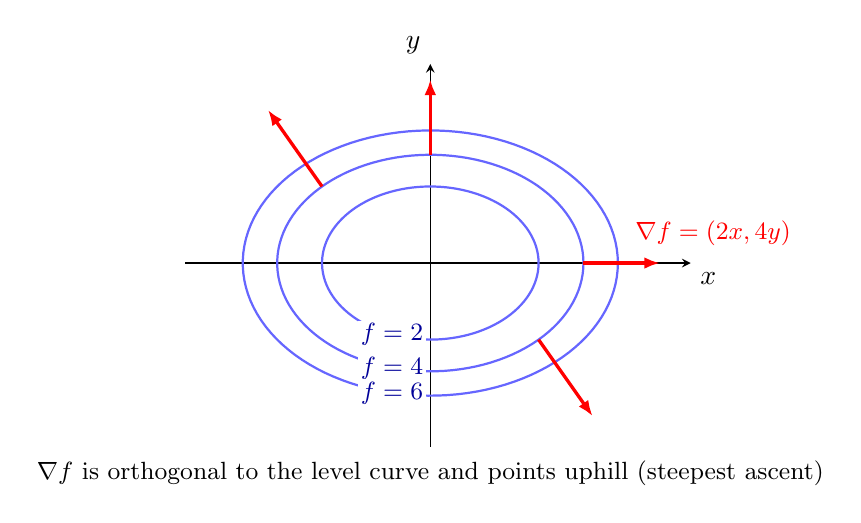
\begin{tikzpicture}
	\begin{axis}[
		axis lines=middle, axis equal image,
		xmin=-3.2, xmax=3.4, ymin=-2.4, ymax=2.6,
		xtick=\empty, ytick=\empty,
		xlabel={$x$}, ylabel={$y$},
		xlabel style={below right}, ylabel style={above left},
		clip=false, width=8cm
		]
		\foreach \c in {1,2,3} {
			\addplot[blue!60, thick, domain=0:360, samples=120] ({sqrt(\c*2)*cos(x)}, {sqrt(\c)*sin(x)});
		}
		\node[blue!60!black, font=\small, fill=white, inner sep=1pt] at (axis cs:-0.5,-0.935) {$f=2$};
		\node[blue!60!black, font=\small, fill=white, inner sep=1pt] at (axis cs:-0.5,-1.369) {$f=4$};
		\node[blue!60!black, font=\small, fill=white, inner sep=1pt] at (axis cs:-0.5,-1.696) {$f=6$};
		% gradient (2x, 4y) scaled 0.25 at points on f=4: (2,0),(0,sqrt2),(-1.414,1)
		\draw[-{Latex[length=2mm]}, red, very thick] (axis cs:2,0) -- (axis cs:3.0,0);
		\draw[-{Latex[length=2mm]}, red, very thick] (axis cs:0,1.414) -- (axis cs:0,2.4);
		\draw[-{Latex[length=2mm]}, red, very thick] (axis cs:-1.414,1) -- (axis cs:-2.12,2.0);
		\draw[-{Latex[length=2mm]}, red, very thick] (axis cs:1.414,-1) -- (axis cs:2.12,-2.0);
		\node[red, anchor=south west, font=\small] at (axis cs:2.55,0.1) {$\nabla f=(2x,4y)$};
		\node[anchor=north, font=\small] at (axis cs:0,-2.45) {$\nabla f$ is orthogonal to the level curve and points uphill (steepest ascent)};
	\end{axis}
\end{tikzpicture}
\end{document}
